% ---------------------------------------------------------------------------------------------------------------
%                       TEMPLATE PARA TRABALHO DE CONCLUSÃO DE CURSO
% ---------------------------------------------------------------------------------------------------------------
% Projeto Original: Template com Customização da classe abnTeX2 para as normas da UTFPR 
% Autores: Diego Marczal
% 	       Michael Vornes <https://github.com/mvornes>
%
% Modificado por: Gabriel Cabral
%----------------------------------------------------------------------------------------------------------------
% Codificação: UTF-8
% LaTeX:  abnTeX2
% ---------------------------------------------------------------------------------------------------------------

% ---------------------------------------------------------------------------------------------------------------
%                                          CARREGA CLASSE PERSONALIZADA
% ---------------------------------------------------------------------------------------------------------------
\documentclass[%twoside,                   % Impressão em frente e verso
    	        oneside,                   % Impressão apenas frente
]{configuracoes/norma-abntex2}

% ---------------------------------------------------------------------------------------------------------------
%                                        INCLUI ARQUIVOS DE CONFIGURAÇÕES
% ---------------------------------------------------------------------------------------------------------------
% ----------------------------------------------------------------------------
%                                   REFERÊNCIAS
% ----------------------------------------------------------------------------
\usepackage[%
    alf,
    abnt-emphasize=bf,
    bibjustif,
    recuo=0cm,
    abnt-url-package=url,       % Utiliza o pacote url
    abnt-refinfo=yes,           % Utiliza o estilo bibliográfico abnt-refinfo
    abnt-etal-cite=1,
    abnt-etal-list=0,
    abnt-etal-text=it,           % Deixa expressao et al em italico
    abnt-thesis-year=final
]{abntex2cite}                  % Configura as citações bibliográficas conforme a norma ABNT

% ----------------------------------------------------------------------------
%                                    PACOTES
% ----------------------------------------------------------------------------

% Codificação e Fonte
\usepackage[utf8]{inputenc}             % Codificação do documento
\usepackage[T1]{fontenc}                % Seleção de código de fonte
\usepackage{times}                      % Usa a fonte Times
%\usepackage[scaled]{helvet}            % Usa a fonte Helvetica
%\usepackage{palatino}                  % Usa a fonte Palatino
%\usepackage{lmodern}                   % Usa a fonte Latin Modern
\usepackage{ae, aecompl}                % Fontes de alta qualidade
\usepackage{latexsym}                   % Símbolos matemáticos
\usepackage{icomma}                     % Uso de vírgulas em expressões matemáticas
\usepackage{microtype}                  % Melhora a justificação do documento

% Tabelas e Imagens
\usepackage{booktabs}                   % Réguas horizontais em tabelas
\usepackage{color, colortbl}            % Controle das cores
\usepackage{float}                      % Necessário para tabelas/figuras em ambiente multi-colunas
\usepackage{graphicx, caption}          % Inclusão de gráficos e legenda
\usepackage{lscape}                     % Permite páginas em modo "paisagem"

% Matemática
\usepackage[tbtags]{amsmath}
\usepackage{amsfonts, amssymb}
\usepackage{subeqnarray}                % Permite subnumeração de equações
\usepackage[algoruled, portuguese]{algorithm2e}  % Permite escrever algoritmos em português
\usepackage{regexpatch}                 % Patching comandos LaTeX

% Estilo e Formatação
\usepackage{indentfirst}                % Indenta o primeiro parágrafo de cada seção
\usepackage{fancyhdr}                   % Cabeçalhos e rodapés personalizados
\usepackage{titlesec}                   % Controle de títulos de seção
\usepackage{varwidth}                   % Ajuste do tamanho da caixa

% Outros
\usepackage{lastpage}                   % Para encontrar última página do documento
\usepackage{verbatim}                   % Apresentar texto como escrito no documento
\usepackage{lipsum}                     % Geração de texto de preenchimento
\usepackage{tocloft}                    % Personalizar formatação de listas
\usepackage{etoolbox}                   % Ferramentas para manipulação de comandos
\usepackage[nameinlink,capitalize]{cleveref} % Referências cruzadas inteligentes
\usepackage{pdfpages}                   % Inclui documentos PDF externos
% ----------------------------------------------------------------------------
%                    CONFIGURAÇÕES DE APARÊNCIA DO PDF FINAL
% ----------------------------------------------------------------------------
\makeatletter
\hypersetup{%
    portuguese,
    colorlinks=false,  % Define se os "links" ficarão coloridos
    linkcolor=blue,    % Define cor dos "links" internos
    citecolor=blue,    % Define cor dos "links" para as referências bibliográficas
    filecolor=blue,    % Define cor dos "links" para arquivos
    urlcolor=blue,     % Define a cor dos "hiperlinks"
    breaklinks=true,   % Ativa quebra de links longos em várias linhas
    pdftitle={\@title},
    pdfauthor={\@author},
    pdfkeywords={abnt, latex, abntex, abntex2}
}
\makeatother
\makeindex % Cria indice remissivo

% ----------------------------------------------------------------------------
%                           OUTRAS CONFIGURACOES
% ----------------------------------------------------------------------------

% Renomeação de Labels para Referências Cruzadas
\renewcommand{\algorithmautorefname}{Algoritmo}
\def\equationautorefname~#1\null{Equa\c c\~ao~(#1)\null}

\crefname{chapter}{Cap.}{Caps.}
\Crefname{chapter}{Capítulo}{Capítulos}

\crefname{section}{Sec.}{Sec.}
\Crefname{section}{Seção}{Seções}

\crefname{subsection}{Subsec.}{Subsec.}
\Crefname{subsection}{Subseção}{Subseções}

\crefname{table}{Tab.}{Tabs.}
\Crefname{table}{Tabela}{Tabelas}

% Hifenização de palavras que não estão no dicionário
\hyphenation{%
    qua-dros-cha-ve
    Kat-sa-gge-los
}

\newcolumntype{M}[1]{>{\centering\arraybackslash}m{#1}} % Centralizar conteúdo da célula

\captionsetup{font=small, singlelinecheck=true, skip = -1pt} % Configura a legenda dos elementos dos /dados

\allowdisplaybreaks % Permite quebra de página no ambiente align


% ---------------------------------------------------------------------------------------------------------------
%                                 INCLUI ARQUIVOS DO TRABALHO DE CONCLUSÃO DE CURSO
% ---------------------------------------------------------------------------------------------------------------

% Insere capa e folha de rosto
% ----------------------------------------------------------------------------
%                                   CAPA
% ----------------------------------------------------------------------------
% Caso algum dos campos não se aplique ao seu trabalho, como por exemplo,
% se não houve coorientador, apenas deixe vazio.
% Exemplos:
% \coorientador{}
% \departamento{}

% ----------------------------------------------------------------------------
%                               DADOS DO TRABALHO
% ----------------------------------------------------------------------------
\titulo{Reconhecimento e Tradu\c{c}\~ao de Frases em LIBRAS Utilizando Redes Neurais}
\subtitulo{\textnormal{}}
\autor{TALES LIMA DE OLIVEIRA}
\autorcitacao{OLIVEIRA, Tales} % Sobrenome em maiúsculo
\local{Brasília}
\data{2024}
\projeto{Trabalho}
\tituloAcademico{Bacharel em Ci\^encia da Computa\c{c}\~ao}

% ----------------------------------------------------------------------------
%                               DADOS DA INSTITUIÇÃO
% ----------------------------------------------------------------------------
\instituicao{Instituto Federal de Brasília}
\departamento{\textit{Campus} Taguatinga}
\programa{Bacharelado em Ci\^encia da Computa\c{c}\~ao}
\logoinstituicao{0.15}{dados/figuras/ifb-logo.png}

% ----------------------------------------------------------------------------
%                              DADOS DOS ORIENTADORES
% ----------------------------------------------------------------------------
\orientador[Orientador:]{Prof. Dr. Raimundo Cláudio da Silva Vasconcelos} 
\instOrientador{Instituto Federal de Brasília - Campus Taguatinga}

%\coorientador[Coorientador:]{A DEFINIR}
%\instCoorientador{Instituto Federal de Brasília - Campus Taguatinga}

% Quando existir mais de um coorientador
% \coorientador[Coorientadores:]{Prof. Me. XXXXXX \newline
% Universidade XXXXXX - Câmpus XXXXXX \newline
% \newline Prof. Dr. XXXXXX. 
% \newline Universidade XXXXXX - Câmpus XXXXXX}

% ----------------------------------------------------------------------------
%                              FOLHA DE ROSTO
% ----------------------------------------------------------------------------

\renewcommand{\folhaderostoname}{FOLHA DE ROSTO}

\preambulo{{\imprimirprojeto} apresentado ao curso de {\imprimirprograma} do {\imprimirinstituicao} do {\imprimirdepartamento}, como requisito parcial para a obtenção do título de {\imprimirtituloAcademico}.}



% -----------------------------------------------------------------------------
%                         FOLHA DE APROVAÇÃO TEMPORÁRIA
% -----------------------------------------------------------------------------

% Você pode utilizar este modelo até a aprovação do trabalho. Após isso, substitua 
% essa folha pela página assinada pela banca.
% Basta substituir o comando \imprimirfolhadeaprovacao{} no documento principal.tex
% pelo comando: \includepdf{folha-aprovacao.pdf}

\dataaprovacao{DIA de MÊS de ANO}

\bancamembrodois{A DEFINIR}
\instbancamembrodois{Departamento de Computação/IFB}

\bancamembrotres{A DEFINIR}
\instbancamembrotres{Departamento de Computação/IFB}

\bancasuplente{A DEFINIR}
\instbancamembrosuplente{Departamento de Computação/IFB}


\begin{document}

    \pretextual
    \imprimircapa                                     % Comando para imprimir Capa
    \imprimirfolhaderosto{}                           % Comando para imprimir Folha de rosto
    %\includepdf{ficha-catalografica.pdf}             % Comando para inserir Ficha catalográfica
    \imprimirfolhadeaprovacao{}                       % Comando para imprimir Folha de aprovação temporária
    
    % Insere elementos pré-textuais
    %% ----------------------------------------------------------------------------
%                               DEDICATÓRIA
% ----------------------------------------------------------------------------

\renewcommand{\dedicatorianame}{DEDICATÓRIA}

\begin{dedicatoria}

    Altere este texto inserindo a dedicatória do seu trabalho. 

\end{dedicatoria}
          		% Dedicatória
    % ----------------------------------------------------------------------------
%                               AGRADECIMENTOS
% ----------------------------------------------------------------------------

\begin{agradecimentos}[AGRADECIMENTOS]

    Agradeço aos meus pais e amigos pelo constante apoio e incentivo durante toda a minha jornada acadêmica.. 
    
    Meu sincero agradecimento ao meu orientador, \imprimirorientador, pela orientação, paciência e por compartilhar seu conhecimento ao longo do desenvolvimento deste trabalho. Sou também grato a todos os professores do \imprimirinstituicao, que contribuíram de maneira significativa para a minha formação.

    Por fim, a todos que, direta ou indiretamente, apoiaram a realização deste trabalho, deixo aqui minha gratidão.

\end{agradecimentos}
        		% Agradecimentos
    % ----------------------------------------------------------------------------
%                                   EPÍGRAFE
% ----------------------------------------------------------------------------

\renewcommand{\epigraphname}{EPÍGRAFE}

\begin{epigrafe}

    \textit{``And in the end, the love you take is equal to the love you make.''}\\
    \textbf{— The Beatles, The End, 1969}

\end{epigrafe}

              		% Epígrafe
    % ----------------------------------------------------------------------------
%                                   RESUMO
% ----------------------------------------------------------------------------

\begin{resumo}[RESUMO]

    \begin{SingleSpacing}

        Este projeto prop\~oe o desenvolvimento de uma rede neural convolucional profunda (DCNN) para reconhecer e traduzir gestos e frases completas em Lingua Brasileira de Sinais (LIBRAS). \\
        
        \textbf{Palavras-chave}: LIBRAS. Rede Neural Convolucional. Vis\~ao Computacional.
    
    \end{SingleSpacing}
    
\end{resumo}
             		% Resumo em Português
    % ----------------------------------------------------------------------------
%                                  ABSTRACT
% ----------------------------------------------------------------------------

\begin{resumo}[ABSTRACT]

    \begin{SingleSpacing}
    
        This project proposes the development of a deep convolutional neural network (DCNN) to recognize and translate gestures and complete sentences in Brazilian Sign Language (LIBRAS). \\

        \textbf{Keywords}: LIBRAS. Convolutional Neural Network. Computer Vision.
    
    \end{SingleSpacing}
    
\end{resumo}
             		% Resumo em Inglês
    % ----------------------------------------------------------------------------
%                           LISTA DE FIGURAS
% ----------------------------------------------------------------------------
% Este arquivo não precisa ser alterado, pois a lista é gerada automaticamente.

\pdfbookmark[0]{\listfigurename}{lof}
\listoffigures*
\cleardoublepage       % Lista de Figuras
    % ----------------------------------------------------------------------------
%                              LISTA DE QUADROS
% ----------------------------------------------------------------------------
% Este arquivo não precisa ser alterado, pois a lista é gerada automaticamente.

\renewcommand{\listofquadrosname}{LISTA DE QUADROS}

\pdfbookmark[0]{\listofquadrosname}{loq}
\listofquadros*
\cleardoublepage
       % Lista de Quadros
    % ----------------------------------------------------------------------------
%                              LISTA DE TABELAS
% ----------------------------------------------------------------------------
% Este arquivo não precisa ser alterado, pois a lista é gerada automaticamente.

\pdfbookmark[0]{\listtablename}{lot}
\listoftables*
\cleardoublepage
       % Lista de Tabelas
    % ----------------------------------------------------------------------------
%                       LISTA DE ABREVIATURAS E SIGLAS
% ----------------------------------------------------------------------------
% Altere a lista para definir os acrônimos e siglas utilizados neste trabalho

\begin{siglas}
    \item[ABNT] Associação Brasileira de Normas Técnicas
    \item[LIBRAS] Lingua Brasileira de Sinais
    \item[TCC] Trabalho de Conclusão de Curso
    \item[DCNN] Rede Neural Convolucional Profunda
\end{siglas}
        % Lista de Abreviaturas e Siglas
    %% ----------------------------------------------------------------------------
%                           LISTA DE SÍMBOLOS
% ----------------------------------------------------------------------------
% Altere a lista para definir os símbolos utilizados no trabalho

\begin{simbolos}
    \item[$ \phi_E $] Fluxo elétrico
    \item[$ \varepsilon_0 $] Permissividade elétrica no vácuo
\end{simbolos}
     % Lista de Símbolos
    % ----------------------------------------------------------------------------
%                            LISTA DE ALGORITMOS
% ----------------------------------------------------------------------------
% Este arquivo não precisa ser alterado, pois a lista é gerada automaticamente.

\newcommand{\algoritmoname}{Algoritmo}
\renewcommand{\listalgorithmcfname}{LISTA DE ALGORITMOS}

\floatname{algocf}{\algoritmoname}
\newlistof{listofalgoritmos}{loa}{\listalgoritmoname}
\newlistentry{algocf}{loa}{0}

\counterwithout{algocf}{chapter}
\renewcommand{\cftalgocfname}{\algoritmoname\space}
\renewcommand*{\cftalgocfaftersnum}{\hfill--\hfill}

\pdfbookmark[0]{\listalgorithmcfname}{loa}
\listofalgorithms
\cleardoublepage    % Lista de Algoritmos
    % ----------------------------------------------------------------------------
%                                  SUMÁRIO
% ----------------------------------------------------------------------------
% Este arquivo não precisa ser alterado, pois o sumário é gerado automaticamente.

\setlength\cftchapternumwidth{2em}

\renewcommand{\contentsname}{SUMÁRIO}

\pdfbookmark[0]{\contentsname}{toc}
\tableofcontents*
\cleardoublepage

               		% Sumário
    
    \textual
    % Insere elementos textuais
    % ----------------------------------------------------------------------------
%                                  INTRODUÇÃO
% ----------------------------------------------------------------------------

\chapter{INTRODUÇÃO}
\label{chap:introducao}

O \LaTeX{} é uma ferramenta poderosa e flexível para criar textos de alta qualidade. Ele oferece um ambiente organizado para produzir documentos acadêmicos bem formatados, permitindo que você se concentre no conteúdo e na pesquisa, enquanto a formatação é cuidada automaticamente.
                		         % Introdução
    % ----------------------------------------------------------------------------
%                           FUNDAMENTAÇÃO TEÓRICA
% ----------------------------------------------------------------------------

\chapter{FUNDAMENTAÇÃO TEÓRICA}
\label{chap:fundamentacaoTeorica}

Este documento é um \emph{template} \LaTeX{} que foi concebido, primariamente, para ser utilizado na elaboração de Trabalho de Conclusão de Curso seguindo as normas da ABNT. Para isso, utilizamos a classe {\ttfamily abntex2.cls}.           % Fundamentação teórica
    % ----------------------------------------------------------------------------
%                               METODOLOGIA
% ----------------------------------------------------------------------------

\chapter{METODOLOGIA}
\label{chap:metodologia}

O arquivo de partida é denominado {\ttfamily principal.tex}. Este \emph{template} está organizado em três diretórios principais: a pasta {\ttfamily /configuracoes}, que contém configurações relacionadas à classe abn\TeX{}2, configurações de saída do PDF e a lista de pacotes empregados; o diretório {\ttfamily /dados}, onde é recomendado organizar Algoritmos, Figuras, Quadros e Tabelas utilizados no trabalho; e a pasta {\ttfamily /estrutura}, que possui os arquivos onde o TCC deve ser redigido.             % Metodologia
    % ----------------------------------------------------------------------------
%                                  RESULTADOS
% ----------------------------------------------------------------------------

\chapter{RESULTADOS E DISCUSSÃO}
\label{chap:resultadosDiscussao}

Antes de começar a escrever o seu trabalho acadêmico utilizando este \emph{template}, é importante editar os arquivos que estão os elementos pré-textuais do trabalho.
São eles os arquivos {\ttfamily capa.tex} e {\ttfamily folha-aprovacao.tex}, localizados no diretório  {\ttfamily /estrutura/pre-textuais}.              % Resultados
    % ----------------------------------------------------------------------------
%                               ORIENTAÇÕES GERAIS
% ----------------------------------------------------------------------------
\chapter{ORIENTAÇÕES GERAIS}
\label{chap:orientacoesGerais}

Neste capítulo são abordados detalhadamente os comandos para formatar o texto, criar listas, tabelas e figuras, inserir equações matemáticas, gerenciar referências bibliográficas.

% ----------------------------------------------------------------------------
%                                FORMATAÇÃO DE TEXTO
% ----------------------------------------------------------------------------
\section{Formatação de Texto}
\label{sec:formatacaoTexto}

\begin{itemize}
    \item \textbf{Negrito e Itálico:} Utilize os comandos \verb|\textbf{}| para negrito e \verb|\textit{}| para itálico. Exemplo: \textbf{texto em negrito} e \textit{texto em itálico}.
    
    \item \textbf{Aspas}: A palavra deve estar entre ``aspas simples duplas''.
    
    \item \textbf{Alinhamento do Texto:} Use \verb|\centering| para centralizar o texto, \verb|\raggedright| para alinhar à esquerda e \verb|\raggedleft| para alinhar à direita.
    
    \item \textbf{Parágrafos e Espaçamento:} Para criar novos parágrafos, deixe uma linha em branco.
    
    \item \textbf{Recuo de Parágrafo:} Se desejar evitar o recuo em um novo parágrafo, utilize o comando \verb|\noindent| no início.
    
    \item \textbf{Quebras de Linha e Página:} Para quebrar linhas, utilize \verb|\\| e \verb|\newline|. Para quebrar páginas, utilize \verb|\newpage|.
    
    \item \textbf{Comentários:} Utilize \verb|%| para fazer comentários no código LaTeX. Para comentários longos utilize  \verb|\begin{comment} ... \end{comment}|.
    % Você pode deixar comentários para quem for ler seu código ou para servir como suas anotações ao longo do texto.
    
    \item \textbf{Espaços:} Utilize \verb|~| para criar espaços não quebráveis.

\end{itemize}

% ----------------------------------------------------------------------------
%                                   LISTAS 
% ----------------------------------------------------------------------------
\section{Listas}
\label{sec:listas}

Em documentos \LaTeX, podemos criar listas não numeradas e numeradas utilizando os ambientes \verb|itemize| e \verb|enumerate|, respectivamente.

\subsection{Listas não numeradas}
\label{subsec:listasNaoNumeradas}
\noindent
Para criar listas não numeradas, use o ambiente \verb|itemize| e marque cada item com \verb|\item|.

\begin{quadro}[!htb]
    \centering
    \begin{tabular}{p{7.5cm}|p{7.5cm}}
        \textbf{Exemplo} & \textbf{Resultado} \\
        
        \begin{verbatim}
        \begin{itemize}
        \item Item 1
        \item Item 2
        \end{itemize}
        \end{verbatim} 
        & 
        \begin{itemize}
        \item Item 1
        \item Item 2
        \end{itemize}
        \\
        
    \end{tabular}
\end{quadro}



\subsection{Listas numeradas}
\label{subsec:listasNumeradas}
\noindent
Para criar listas numeradas, use o ambiente \verb|enumerate| e marque cada item com \verb|\item|.

\begin{quadro}[!htb]
    \centering
    \begin{tabular}{p{7.5cm}|p{7.5cm}}
        \textbf{Exemplo} & \textbf{Resultado} \\
        
        \begin{verbatim}
        \begin{enumerate}
        \item Item 1
        \item Item 2
        \end{enumerate}
        \end{verbatim}
        & 
        \begin{enumerate}
        \item Item 1
        \item Item 2
        \end{enumerate}
        \\
        
    \end{tabular}
\end{quadro}



% ----------------------------------------------------------------------------
%                                   CITAÇÕES 
% ----------------------------------------------------------------------------
\section{Citações}
\label{sec:citacoes}

Nesta seção, vamos abordar como fazer citações diretas e indiretas utilizando os comandos \LaTeX{} apropriados.

\subsection{Citação indireta}
\label{subsec:citacaoIndireta}

A citação indireta é a transcrição das ideias de um autor, utilizando suas próprias palavras, mas mantendo o sentido original. Para fazer uma citação indireta, utilize os comandos \verb|\cite{chave}| e \verb|\citeonline{chave}|, colocando entre as chaves o nome do autor ou o identificador da referência bibliográfica.

\textbf{Exemplos:}
\begin{itemize}
    \item  Uma compreensão física é uma coisa completamente não-matemática, imprecisa e inexata, mas absolutamente necessária para um físico \cite{feynman}.
    \item Para \citeonline{feynman}, os físicos precisam ter flexibilidade para olhar os problemas sob diversos pontos de vista.
\end{itemize}

\subsection{Citação direta}
\label{subsec:citacaoDireta}

Quando o trecho citado é longo (4 ou mais linhas) deve-se usar um parágrafo específico para a citação, na forma de um texto recuado (4 cm da margem esquerda), com tamanho de letra menor e espaçamento entrelinhas simples. Exemplo de citação longa:
\\
\begin{citacao}
    Para qualquer campo eletrostático, não existe nenhum ponto de equilíbrio estável – exceto exatamente sobre uma outra carga. Usando a lei de Gauss, é fácil ver a razão disto. Primeiro, para uma carga estar em equilíbrio em qualquer ponto particular $P_0$, o campo ali deve ser zero. Segundo, para que este equilíbrio seja estável, devemos exigir que, se afastarmos a carga de $P_0$ em qualquer direção, surja uma força restauradora direcionada em oposição ao deslocamento. O campo elétrico em todos os pontos vizinhos deve apontar na direção de $P_0$. Mas, como podemos ver facilmente, se não existir nenhuma carga em $P_0$ isto é uma violação da lei de Gauss \cite[p.~51]{feynman}.

   % Desse modo, opera-se uma ruptura decisiva entre a reflexividade filosófica, isto é a possibilidade do sujeito de pensar e de refletir, e a objetividade científica. Encontramo-nos num ponto em que o conhecimento científico está sem consciência. Sem consciência moral, sem consciência reflexiva e também subjetiva. Cada vez mais o desenvolvimento extraordinário do conhecimento científico vai tornar menos praticável a própria possibilidade de reflexão do sujeito sobre a sua pesquisa \cite[p.~28]{Silva2000}.
\end{citacao}
\noindent
Para fazer a citação longa deve-se utilizar os seguintes comandos:
\begin{verbatim}
    \begin{citacao}
    <texto da citacao>
    \end{citacao}
\end{verbatim}

No exemplo acima, para a chamada da referência o comando \verb|\cite[p.~28]{Silva2000}| foi utilizado, visto que os nomes dos autores não são parte do trecho citado. É necessário também indicar o número da página da obra citada que contém o trecho citado.

% ----------------------------------------------------------------------------
%                              REFERÊNCIAS CRUZADAS
% ----------------------------------------------------------------------------
\section{Referências Cruzadas}
\label{sec:referenciasCruzadas}

As referências cruzadas são uma funcionalidade essencial no \LaTeX{}, permitindo criar conexões automáticas entre diferentes partes do documento, como capítulos, seções, figuras, tabelas, equações e outros elementos numerados. Para utilizar referências cruzadas, é necessário incluir um rótulo ({\ttfamily label}) em cada elemento que se deseja referenciar.

\subsection{Inserindo um Rótulo}
Para criar um rótulo, utilize o comando \verb|\label{nome}| no local desejado. O \verb|nome| é um identificador único que você atribui ao elemento. É recomendável utilizar nomes descritivos, como \verb|chap:introducao| para um capítulo ou \verb|fig:exemplo| para uma figura. 

\textbf{Exemplo:}
\begin{verbatim}
    \section{Listas}
    \label{sec:listas}
\end{verbatim}

\subsection{Referenciando um Elemento}
Para fazer referência a um elemento previamente rotulado, utilize os comandos \verb|\ref{nome}|, \verb|\autoref{nome}| ou \verb|\cref{nome}|. O comando \verb|\ref{nome}| simplesmente mostra o número do elemento referenciado, o comando \verb|\autoref{nome}| adiciona automaticamente o tipo do elemento (como ``Capítulo'', ``Figura'', ``Equação'', etc.) antes do número, enquanto \verb|\cref{nome}| é similar ao comando anterior, mas o tipo do elemento é abreviado (como ``Cap.'', ``Fig.'', ``Eq.'', etc.).

\textbf{Exemplo:}
\begin{verbatim}
    Na \autoref{sec:listas} são abordadas informações sobre listas no documento.
\end{verbatim}

\textbf{Resultado:} \\
``Na \autoref{sec:listas} são abordadas informações sobre listas no documento.''

\subsection{Elementos com rótulos}
Aqui estão alguns elementos comuns que podem receber rótulos para referências cruzadas:
\begin{itemize}
    \item Capítulos: \texttt{\textbackslash chapter\{...\}\textbackslash label\{chap:nome\}}
    \item Seções: \texttt{\textbackslash section\{...\}\textbackslash label\{sec:nome\}}
    \item Subseções: \texttt{\textbackslash subsection\{...\}\textbackslash label\{subsec:nome\}}
    \item Figuras: \texttt{\textbackslash begin\{figure\}...\textbackslash caption\{...\}\textbackslash label\{fig:nome\}\textbackslash end\{figure\}}
    \item Tabelas: \texttt{\textbackslash begin\{table\}...\textbackslash caption\{...\}\textbackslash label\{tab:nome\}\textbackslash end\{table\}}
    \item Equações: \texttt{\textbackslash begin\{equation\}...\textbackslash label\{eq:nome\}\textbackslash end\{equation\}}
\end{itemize}
\vspace{0.5cm}
Com o uso adequado de rótulos e referências cruzadas, você pode criar um documento bem estruturado e de fácil navegação no \LaTeX{}. 

% ----------------------------------------------------------------------------
%                                   FIGURAS
% ----------------------------------------------------------------------------
\section{Figuras}
\label{sec:figuras}

Exemplo de como inserir a \autoref{fig:figura-exemplo-1}, que pode ser referenciado como \cref{fig:figura-exemplo-1}. As figuras aparecem automaticamente na lista de figuras. Os arquivos das imagens devem ser armazenados no diretório de ``/dados''.

\begin{figure}[!htb]
    \centering
    \caption{Possíveis distribuições de cargas em uma superfície de espessura não nula.}
    \sbox0{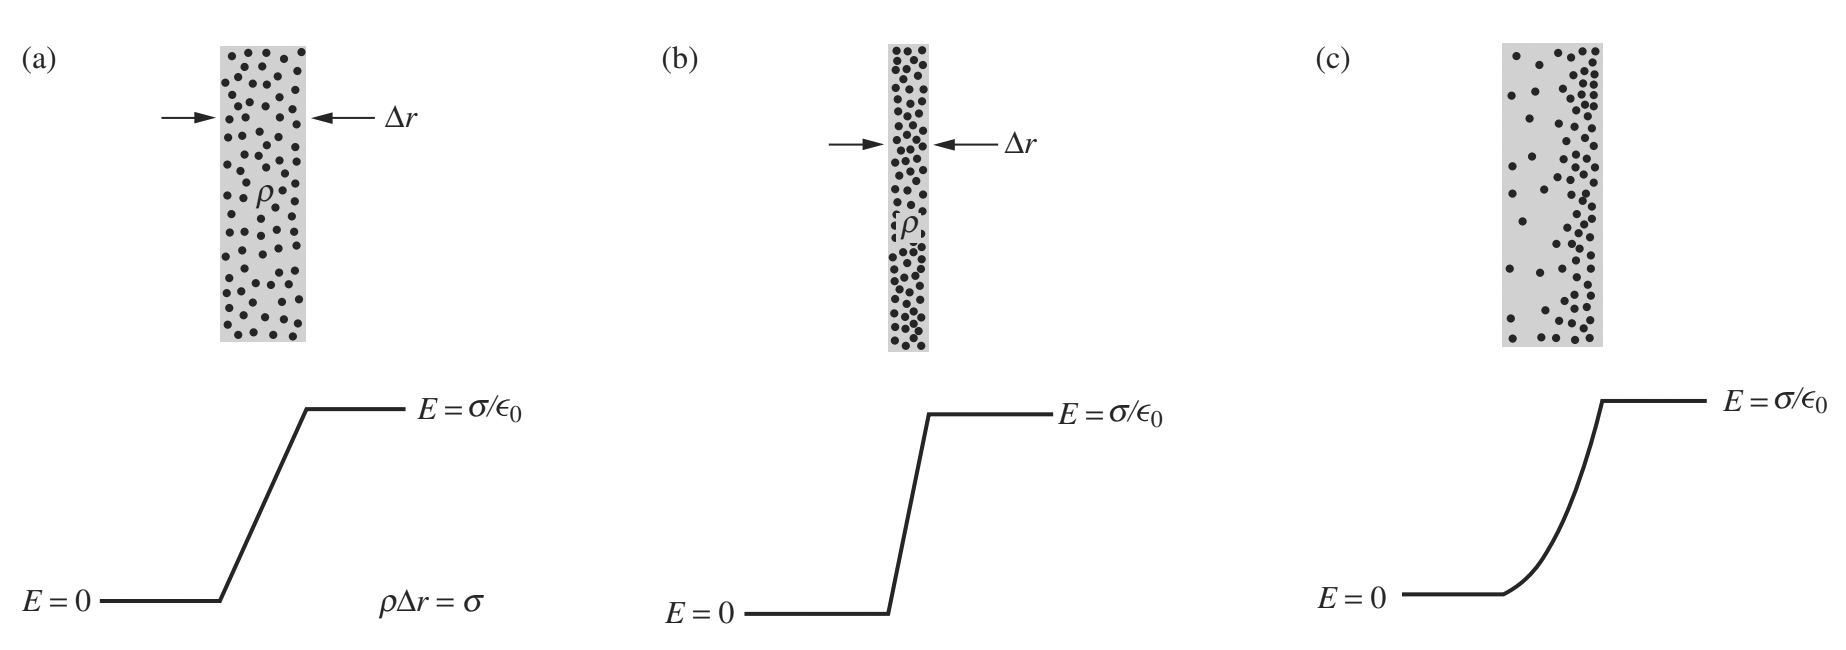
\includegraphics[width=0.8\textwidth]{./dados/figuras/purcell}}
    \begin{minipage}{\wd0}
        \usebox0
        \vspace{-20pt}
        \label{fig:figura-exemplo-1}
        \fonte{\citeonline[p.~31]{purcell}.}
    \end{minipage}
\end{figure}

% ----------------------------------------------------------------------------
%                                QUADROS E TABELAS
% ----------------------------------------------------------------------------
\section{Quadros e tabelas}
\label{sec:quadrosTabelas}

Exemplo de como inserir o \autoref{qua:quadro-exemplo1} e a \cref{tab:tabela-exemplo1}. Ambos aparecem automaticamente nas suas respectivas listas.
Os elementos (Quadros e Tabelas) devem ser criados em arquivos separados para facilitar manutenção e armazenados no diretório de ``/dados".

\begin{quadro}[!htb]
    \centering
    \caption{Campo elétrico produzido por distribuição esférica de carga.\label{qua:quadro-exemplo1}}
    \begin{tabular}{|p{5cm}|p{4.8cm}|p{4.8cm}|}
        \hline
        \textbf{Distribuição de cargas} & \textbf{Ponto em campo elétrico} & \textbf{Módulo do campo elétrico} \\
        \hline
        Carga $q$ sobre a superfície de uma esfera condutora com o raio $R$. & 
        
        Fora da esfera, $r > R$ \newline \newline
        Dentro da esfera, $r < R$ & 
        
        $E = \frac{1}{4\pi\varepsilon_0} \frac{Q}{r^2}$ \newline \newline
        $E = 0$
        \\
        \hline
    \end{tabular}
    \fonte{\citeonline{young}.}
\end{quadro}


A diferença entre quadro e tabela está no fato que um quadro é formado por linhas horizontais e verticais. Deve ser utilizado quando o conteúdo é majoritariamente não-numérico. Uma tabela é formada apenas por linhas verticais, e deve ser utilizada quando o conteúdo é majoritariamente numérico.

\begin{table}[!htb]
    \centering
    \caption{Algumas propriedades elétricas do cobre e do silício. \label{tab:tabela-exemplo1}}
    \begin{tabularx}{\textwidth}{lcc}
        \toprule
            Propriedade                                            & Cobre & Silício      \\ 
        \midrule
            % Tipo de material                                       & Metal & Semicondutor \\
            Densidade de portadores de carga, $m^{-3}$             & $\mathrm{8,49} \times 10^{28}$ & $\mathrm{1} \times 10^{16}$     \\
            Resistividade, $\Omega \cdot m$                        & $\mathrm{1,69} \times 10^{-8}$  & $\mathrm{2,5} \times 10^{3}$   \\
            Coeficiente de temperatura da resistividade, $K^{-1}$  & $\mathrm{+4,3} \times 10^{-3}$  & $\mathrm{-70} \times 10^{-3}$  \\ 
        \bottomrule
    \end{tabularx}
    \fonte{\citeonline{halliday}.}
\end{table}

% ----------------------------------------------------------------------------
%                                  EQUAÇÕES
% ----------------------------------------------------------------------------
\section{Equações}
\label{sec:equacoes}

Exemplo de como inserir a \autoref{eq:equacao-exemplo1} e a \cref{eq:equacao-exemplo2} no corpo do texto. Observe que foram utilizadas duas formas distintas para referenciar as equações. O comando \verb|\ref{nome}| também é válido para exibir apenas o número da equação.

\begin{equation}
    \label{eq:equacao-exemplo1}
    f(x) = \frac{a_0}{2} + \sum_{n=1}^{\infty} \left[a_n \cos{ \left( \frac{ n\pi x}{L} \right) }  +  b_n  \: \mathrm{sen}{ \left( \frac{ n\pi x}{L} \right) }     \right]
    ,
\end{equation}

\begin{align}
    \phi_E  = \int \limits_{A} \Vec{E_1}\cdot (-\Hat{n}) \, dA'\ + \int \limits_{A} \Vec{E_2}\cdot \Hat{n} \, dA'\
    \label{eq:equacao-exemplo2}
\end{align}
\noindent
A numeração das equações é inserida e atualizada automaticamente. É possível remover o número de uma equação ao adicionar um asterisco no parâmetro  {\ttfamily equation}, como em

\begin{equation*}
    \oint \limits_S \Vec{E}\cdot d \Vec{A}\ =
    \frac{Q_{\mathrm{enc}}}{\varepsilon_0}
    .
\end{equation*}

Existem outros parâmetros para inserir equações, como o {\ttfamily align},  {\ttfamily split}.
Além disso, o ambiente matemático pode ser utilizado ao longo do texto ao envolver a equação com cifrão (\$). Por exemplo, como feito com a equação $ dE_x = dE \cos\theta $.

% ----------------------------------------------------------------------------
%                                   ALGORITMOS
% ----------------------------------------------------------------------------
\section{Algoritmos}
\label{sec:algoritmos}

Exemplo de como inserir um algoritmo. Para inserção de algoritmos utiliza-se o pacote {\ttfamily algorithm2e} que já está devidamente configurado dentro do template.
Os algoritmos devem ser criados em arquivos separados para facilitar manutenção e armazenados no diretório de ``/dados''. \\
\begin{algorithm}
    \caption{Algoritmo de Fibonacci Recursivo: $O(2^n)$}
    \KwIn{inteiro não negativo $n$}
    \KwOut{valor do $n$-ésimo número de Fibonacci $F(n)$}
    \If{$n \leq 1$}{
        \Return $n$
    }
    \Return $F(n-1) + F(n-2)$
\end{algorithm}

% ----------------------------------------------------------------------------
%                           REFERÊNCIAS BIBLIOGRÁFICAS
% ----------------------------------------------------------------------------
\section{Referências bibliográficas}
\label{sec:referenciasBibliograficas}

A bibliografia é feita no padrão \textsc{Bib}\TeX{}. Para facilitar a manutenção, as referências são colocadas em um arquivo separado. Neste \textit{template} as referências são armazenadas no arquivo \verb|base-referencias.bib|.

Existem diversas categorias documentos e materiais componentes da bibliografia. A classe abn\TeX{} define as seguintes categorias (entradas):

\begin{verbatim}
@book
@inbook
@article
@phdthesis
@mastersthesis
@monography
@techreport
@manual
@proceedings
@inproceedings
@journalpart
@booklet
@patent
@unpublished
@misc
\end{verbatim}

Cada categoria (entrada) é formatada pelo pacote \citeonline{abnTeX22014d} de uma forma específica. Algumas entradas foram introduzidas especificamente para atender à norma \citeonline{NBR6023:2002}, são elas: \verb|@monography|, \verb|@journalpart|, \verb|@patent|. As demais entradas são padrão \textsc{Bib}\TeX{}.
             % Orientações gerais (remover)
    % ----------------------------------------------------------------------------
%                                 CONCLUSÃO
% ----------------------------------------------------------------------------

\chapter{CONSIDERAÇÕES FINAIS}
\label{chap:conclusao}

Parte final do texto, na qual se apresentam as conclusões do trabalho
acadêmico. É importante fazer uma análise crítica do trabalho, destacando os
principais resultados e as contribuições do trabalho para a área de pesquisa.
                 			     % Conclusão
    
    \postextual
    % Insere elementos pós-textuais
    % ----------------------------------------------------------------------------
%                               REFERÊNCIAS
% ----------------------------------------------------------------------------
% Este arquivo não precisa ser alterado, pois as referências são geradas automaticamente.

\renewcommand{\bibname}{REFERÊNCIAS}

\bibliography{./base-referencias}{} % Carrega o arquivo "base-referencias.bib" e extrai automaticamente as referências citadas
\bibliographystyle{abntex2-alf} % Define o estilo ABNT para formatar a lista de referências
           			   % Referências
    % ----------------------------------------------------------------------------
%                                  APÊNDICES
% ----------------------------------------------------------------------------

\begin{apendicesenv}
    
    % Primeiro apêndice
    \chapter{Nome do apêndice}
    \label{chap:apendiceA}
    
    Caso o material ou texto suplementar ou complementar seja de sua autoria, então ele deverá ser colocado como um apêndice. Porém, caso a autoria seja de terceiros, então o material ou texto deverá ser colocado como anexo.
    
    Caso seja conveniente, podem ser criados outros apêndices para o seu trabalho acadêmico. Basta recortar e colar este trecho neste mesmo documento. Lembre-se de alterar o \textit{label} do apêndice.
    
    
    % Segundo apêndice
    % \chapter{Nome do apêndice B} % Edite para alterar o título deste apêndice
    % \label{chap:apendiceB}
    % Texto
    
\end{apendicesenv}
             			   % Apêndices
    % ----------------------------------------------------------------------------
%                                 ANEXOS
% ----------------------------------------------------------------------------

\begin{anexosenv}

    % Primeiro anexo
    \chapter{Nome do anexo}
    \label{chap:anexoA}
    
    Caso o material ou texto suplementar ou complementar seja de sua autoria, então ele deverá ser colocado como um apêndice. Porém, caso a autoria seja de terceiros, então o material ou texto deverá ser colocado como anexo.
    
    Caso seja conveniente, podem ser criados outros anexos para o seu trabalho acadêmico. Basta recortar e colar este trecho neste mesmo documento. Lembre-se de alterar o \textit{label} do anexo.
    
    
    % Segundo anexo
    % \chapter{Nome do outro anexo}
    % \label{chap:anexoB}
    % Texto

\end{anexosenv}
               			   % Anexos

\end{document}
